\documentclass[11pt]{beamer}

\usepackage{amsmath, graphicx, natbib, verbatim, color}
\usepackage{colortbl}
%\usetheme{CambridgeUS}

\useoutertheme{infolines}
\usetheme{default}

\setbeamertemplate{navigation symbols}{}
\setbeamertemplate{headline}{}


\setbeamertemplate{navigation symbols}{}

\definecolor{forest}{rgb}{.15, .5, .15}
\definecolor{brick}{rgb}{.7, .15, .15}
\definecolor{darkgreen}{rgb}{.15, .5, .15}
\definecolor{darkred}{rgb}{.7, .15, .15}
\definecolor{darkblue}{rgb}{.15, .15, .7}
\definecolor{Green}{rgb}{0.2,1,0.2}

\usepackage[english]{babel}
\usepackage[latin1]{inputenc}
\usepackage{times}
\usepackage[T1]{fontenc}

\usepackage{natbib}
\usepackage{bibentry}
\bibliographystyle{apalike}
% command def below needed on ada distro
%\newcommand{\newblock}{\hskip .11em plus .33em minus .07em}


\setbeamercolor*{bibliography entry title}{fg=black}
\setbeamercolor*{bibliography entry author}{fg=black}
\setbeamercolor*{bibliography entry location}{fg=black}
\setbeamercolor*{bibliography entry note}{fg=black}
\setbeamertemplate{bibliography item}{}

\setbeamertemplate{frametitle continuation}[from second]
\setbeamercovered{transparent}

\setlength{\itemsep}{1.5ex}
\setlength{\parskip}{1.5ex}

% \setlength{\itemsep}{15em}


\title[Clinical Trials \& Survival Analysis]% (optional, with long titles)
{`Recent' History of Survival Analysis in Clinical Trials} 
\author[Harrington] {Dave Harrington
 \texttt{dph@jimmy.harvard.edu} }

\institute % (optional)
[Harvard, DFCI] {{\color{brick} Harvard Statistics and Biostatistics, Dana-Farber Cancer Institute }}

\date{12 August 2015}

%\newcommand*{\refname}{Bibliography}
\begin{document}


\begin{frame}
 
 \titlepage
    
\end{frame}
%--- Next Frame ---%


\begin{frame}{Some Context}

\cite{smith1998clintrials}
    
\begin{quote}
    Was the randomised controlled trial the most
    important development in medicine this [$20^{th}$] century?
    
\end{quote}
    
In T. Jefferson's 1807 letter to Caspar Washington [\cite{jefferson1985letters}]

\begin{quote}
    
    The patient, treated on the fashionable theory, sometimes gets well in
    spite of the medicine. The medicine therefore restored him, and the young
    doctor receives new courage to proceed in his bold experiments on the
    lives of his fellow creatures.
    
\end{quote}
    
    
\textcolor{forest}{All references at the end.  First edition dates used for texts.}

\end{frame}
%--- Next Frame ---%

\begin{frame}[t]{Why link clinical trials and survival analysis?}
	
	
	\begin{center}
	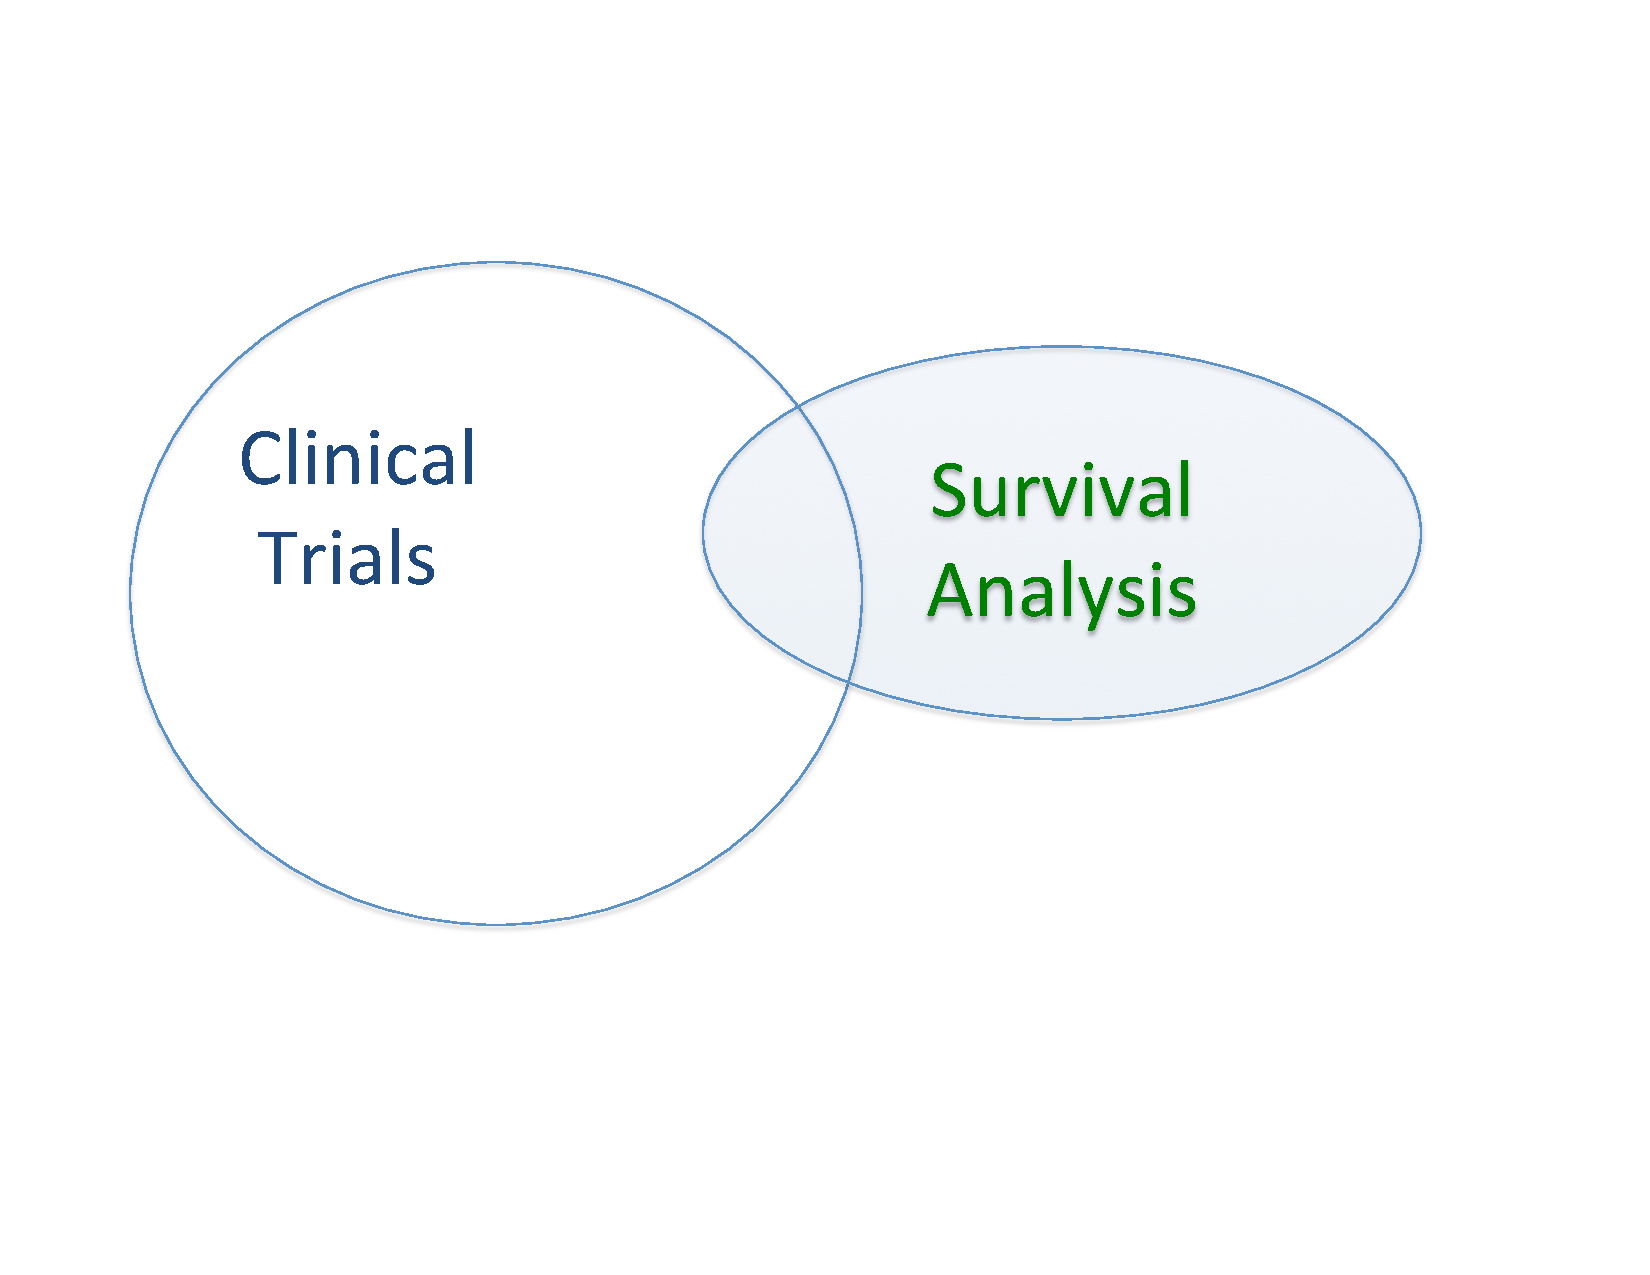
\includegraphics[width= 0.60\textwidth]{clin_surv_venn.pdf}
	\end{center}

\vspace*{-0.5in}

First `modern' randomized clinical trial in 1948 [\cite{marshall1948streptomycin}]

Earliest work in estimating survival distributions seems to be Graunt's 1661 life tables [\cite{graunt2008natural}, Kindle (!) Edition]. 

	\textcolor{forest}{Some important features of survival analysis responded to problems in clinical trials.} 
	

\end{frame}
%--- Next Frame ---%

\begin{frame}{Clinical trials and the shift to non-parametric methods.}
    

The study of reliability produced parametric methods  for estimating life distributions.  From \cite{mann1974methodsfor}:

\begin{quote}
``the probability of a device (or item or organism) performing its (or his or her) defined purpose adequately for a specified period of time, under the operating conditions encountered''
\end{quote}

Early skepticism of modeling in JW Boag's discussion of \cite{armitage1959comparison}.

Difficult to determine when the use of non-parametric survival methods became routine for clinical trials.

	
\end{frame}
	
\begin{frame}{Non-parametric approaches build momentum}	

Early non-parametric approaches:

\begin{itemize}
	\item \cite{berkson1952survival} (estimation)
	
	\item \cite{gehan1965generalized} (testing)
\end{itemize} 

Non-parametrics `flourished' with 
\begin{itemize}
    \item \cite{1958nonpakaplanrametric} ($11^{th}$ most highly cited paper in Web of Science) and 
    
    \item \cite{mantel1966evaluation}, \cite{peto1972asymptotically} 
\end{itemize}

\cite{elveback1958estimation} (118 citations) vs KM (approx 46,000 citations) shows power of marketplace: parametric vs. non-parametric.

\end{frame}


%--- Next Frame ---%

\begin{frame}{More refined analysis of clinical trials}
    
 The early nonparametric approach did not support modeling, adjusting for confounders, etc.
 
 \begin{itemize}

   \item The proportional hazards model and its partial likelihood provided a modeling tool [\cite{cox1972regression}, approx. 40,000 citations, $24^{th}$ most highly cited].
 
 \begin{itemize}
     \item $\lambda(t|z) = \lambda_0(t) \exp(\beta' z)$
     
     \item Contribution to the partial likelihood for $\beta$ at failure time $t_i$
          \[ 
          \frac{\exp(\beta'Z_{(i)})}{\sum_{l \in R_i} \exp(\beta'Z_l)}
     \]
\end{itemize}

\pause

  \item Early hints of the PH model in exponential regression [\cite{feigl1965estimation}].
  
  \item Accelerated failure time model provided an alternative.
  
 \end{itemize}

    
\end{frame}


\begin{frame}{Moving on from 1972}
    
Many wonderful side trips \ldots    
    \begin{itemize}
        \item \cite{buckley1979linear} proposed using linear regression
        
        \item Competing risks, sample size calculations, model checking, interval censored data, examining efficiency, adjusting for tied failure times. %\cite{george1974planning}
        
        
    \end{itemize}
    
   % \end{frame}
    
   %   \begin{frame}
        
 \cite{kalbfleisch1980statistical}, \cite{Miller1981survival}, and \cite{cox1984analysis} provided  important contributions and consolidations.
 
\pause
 
 Some vexing problems in trials: 
 \begin{itemize}
        
        \item Theory lacked the elegance of linear models
        
        \item  Interim monitoring
            
        \item Causal inference in randomized trials with some non-adherence
            
    \end{itemize}
    
\end{frame}
%--- Next Frame ---%

\begin{frame}{First, the mathematics}
    
Heroic efforts to pin down asymptotics using `traditional methods'

\begin{itemize}
    \item Kaplan-Meier product limit estimator: \cite{breslow1974large}, others
    
    \item Proportional hazards model: \cite{tsiatis1981large}, others

    \item Partial likelihood: \cite{efron1977efficiency}, \cite{wong1986theory}
\end{itemize}

\pause

Structure came from surprising source: French school of probability [\cite{meyer1966probability}], via \cite{aalen1978nonparametric}.  Partial likelihood score for $\beta$:

\[
   U(\beta,t) = \sum_i \int_0^t [Z_i(u) - E(\beta, u)]dM_i(u)
\]
  
\end{frame}

\begin{frame}{The mathematics \ldots}
    
Important contributions using the martingale approach:

\begin{itemize}
    \item The Kaplan-Meier estimate and the two sample problem: \cite{gill1980censoring}.
    
    \item The proportional hazards model: \cite{andersen1982cox}
    
    \item A general summary, with many applications \cite{andersen1993statistical}.  Affectionately, \textit{ABGK}
\end{itemize}    
    
Surprisingly useful in exploratory data analysis;  \cite{therneau2000modeling}

Made many difficult problems more accessible, e.g., sequential monitoring

    
\end{frame}

\begin{frame}{Sequential Designs}

Sequential monitoring was a `not so immediate' response to the natural question: can we have a look at the data?

Some of the early work was not survival specific:

\begin{itemize}
    
  \item \cite{armitage1960sequential} important, early work (not survival focused).
  
  \item \cite{haybittle1971repeated}, early group sequential approach.
  
  \item \cite{pocock1977group}, the group sequential approach.
  
  \item \cite{o1979multiple}, for the boundaries most often used today.
  
  \item \cite{lan1983discrete}, flexible computation of boundaries.
  
  \end{itemize}
  
 \pause

\cite{tsiatis1981asymptotic} used counting processes to show that all of the earlier technology could be applied in survival analysis, for commonly used tests.
%% a picture here would be very helpful
    
\end{frame}

\begin{frame}{Causal Inference}
	
Methods for causal inference in observational studies well developed.

What do clinical trials add here?  Immediacy, aversion to models \ldots

\begin{itemize}
	\item A clinical trial disrupted by non-adherence is distressing and expensive.
	
	\item Trialists studying chronic diseases are allergic to fully specified models.
\end{itemize}
   
 
Standard approach: Intent-to-Treat (ITT) in superiority RCTs, Per Protocol (PP) and ITT in non-inferiority RCTs.

Neither approach is very satisfying, despite FDA and EMA endorsement. 

\end{frame}

\begin{frame}{Causal inference \ldots}
	
\cite{imbens2015causal} summarizes theory and applications of the \textsl{Rubin Causal Model}.

\begin{itemize}
	\item Useful for binary or normally distributed `immediate outcomes', not easy to adapt to censored event time data without a parametric model.
\end{itemize}

\cite{robins1991correcting} use Rank Preserving Structural Failure time models, or the structural version of the accelerated failure time model.

\begin{itemize}
	
	\item Inference not based on assumptions about shape of baseline event rate function.
	
	\item Inspired by the prevalence of self-medication in the early days HIV clinical research.
\end{itemize}

Neither approach has substantially penetrated practice.
	
\end{frame}

\begin{frame}{Causal inference \ldots}
	
Some side trips that show promise, but still used more often in observational studies

\begin{itemize}
	\item Principal Stratification: \cite{frangakis2002principal}
	
	\item Instrumental variables: \cite{angrist1996identification} 
	
	\item Propensity scores: \cite{rosenbaum1983central}
\end{itemize}
	
\end{frame}
%--- Next Frame ---%

\begin{frame}{Emerging areas}
    
\begin{itemize}
    \item Adaptive designs.  \cite{tsiatis2003inefficiency} and \cite{gallo2006adaptive} give different views on this.
    
    \item Bayes.  Slightly perverse to cite this as something that is coming. \cite{spiegelhalter1994bayesian} very compelling argument for Bayesian designs and analysis.  \cite{ibrahim2005bayesian} consolidates what was known in 2005.
    
    \item Design and analyses for `targeted' therapies biomarker adaptive designs [\cite{jiang2007biomarker}, \cite{barker2009spy}: I-SPY 2 trial].
    
    \item Patient-level prediction [\cite{graf1999assessment}, \cite{gerds2008performance}].

\end{itemize}
	
\end{frame} 


\begin{frame}[allowframebreaks]
\frametitle{References}
\bibliography{jsm_references}
\end{frame}
\end{document}

Transcript/timing

  -- Title + 13 content slides; 20 mins for talk, approx 1.5 mins per content slide
  
  -- Title slide; thanks for the opportunity; not a historian, so perspective is a mix of personal and lit review; 20 seconds.  Some sweeping generalizations, simplifications should not be taken too seriously.
  
  -- Slide 2: quotes from Smith, Jefferson.  Richard Smith's question rhetorical, Jefferson's anticipatory. 1 minute
  Running time total: 1 min, 20 seconds
  
  -- Slide 3: Why link?  Why talk about the gap? Overlapping topics, size of blobs not accidental.  As an area of research, survival analysis much older. Cite two papers.  Clinical trials is a larger, arguably more important topic.   1 min
  
  -- 4: shift to nonparametrics: 1.5 min  By 1950's use of parametric models with types of censoring widely used in engineering.  But parametric models in study of chronic disease is risky, discussion of risks appear in Boag's discussion of Armitage's paper.  More on next slide. 1.5 min
  
  
  -- 5: Nonparametrics builds momentum: 2 min.  Organize by testing vs estimation.  Berkson/Gage returned to Graunt's work, used conditional prob arguments (look at paper), while KM used ML approach.  Gehan used classical Wilcoxon, Mantel more intuitive.  Interesting counterpoint.  We left the parametric world behind.  Elveback vs KM
  
  From one view, a single idea is at the heart of the KM, Mantel approaches.  Data come from a process, conditioning on current state one can calculate an independent increment for a statistic. More on this later
  
  -- 6. More refined analyses: 2 mins.  Need for more refined analyses in clinical trials and observational studies.  Sir David Cox's paper did that in 72, and is still the most widely used model for survival analysis in chronic diseases.  Why the formula?  Increment to a likelihood like function, also thinking of data (implicitly) as a process.  Zelen Feigl, accelerated failure time model.  Cox model stuck because it was closest to Graunt's approach.  One way to describe a process is the rate at which things are happening.
  
  -- 7. Side trips: 1.2 mins  Interesting sidelights, consolidation, some vexing problems as trials became more complex
  
  -- 8.  First, the math: 2 mins.  Heroic efforts; French school of probability. Ref to Bourbaki.  With the martingale formulation, previous ideas merged, made explicit.  O - E, martingale is independent increments
  
  -- 9.  The mathematics: 1.5 mins
  
  -- 10. Sequential Analysis: 2 mins (run the list). Emphasize that it is difficult to overstate the value of this work.  Lots of work not cited here.
  
  -- 11. Causal inference: 1.5 mina
  
  -- 12. Causal
  
  -- 13. Causal
  
  -- 14. Emerging areas
  
  
  











From JI, regarding Bayes

Dave, lunch is it.

 I think generally speaking, the most important contribution Bayes methods for survival is the ability to fit very complex survival models using MCMC.

Bayes and MCMC have opened the door for doing computationally feasible exact inference and prediction for complex survival models which really could not be well handled before in other paradigms. Such models include joint models for longitudinal and survival data, cure rate models, random coefficient models, frailty models, multivariate survival models, missing data in survival, and now more recently, Bayes methods for clinical trials design with complex survival models.  

 Second, another big door that Bayes has opened is the natural incorporation of historical data into the design and analysis of clinical trials with time to event endpoints as well as binary or other continuous endpoints. The Bayes paradigm allows such a natural incorporation through a prior distribution, which can greatly reduce sample size in the design of a clinical trials and/or produce unbiased and more efficient estimates of treatment effects in survival analysis.

 
Our survival book really tries to hammer these points home in the first chapter in a section called Why Bayes? We can certainly talk more about this if you like.


Attached is a recent review paper that also addresses prior elicitation, Bayes clinical trial design, and survival.

 

Joe

From Andreas Ziegler

Dear Dave,

Many thanks for the slide. I have really enjoyed your talk but I was wondering why you have chosen the 16th century. I would have started with Ulpian (Wikipedia entry: https://en.wikipedia.org/wiki/Ulpian%27s_life_table) who derived some life tables.

I have two other references for you (and one question):

A Medical Research Council Investigation. Streptomycin treatment of pulmonary tuberculosis. BMJ 1948;2:769-82

Medical Research Council. Clinical trial of patulin in the common cold: report of the Patulin Clinical Trials Committee, Medical Research Council. Lancet 1944;ii:373-5

In the German literature on the history of modern clinical trials, these two trials are listed as the first two modern RCTs. Is there are reason why you have chosen just the streptomycin trial and not the Patulin trial?

My favorite article on the history of trials (it is a German one) is available online:
http://www.saez.ch/docs/saez/archiv/de/2005/2005-44/2005-44-868.pdf

I hope that you will summarize your history of survival analysis in clinical trials as a journal article, and I am already looking forward to your manuscript.

Again, I have really enjoyed your presentation, and I would love to read a summary of your work!

With best wishes

Andreas 


